\documentclass{standalone}
\usepackage{pgfplots}
\usepgfplotslibrary{fillbetween}
\usetikzlibrary{patterns}
\begin{document}
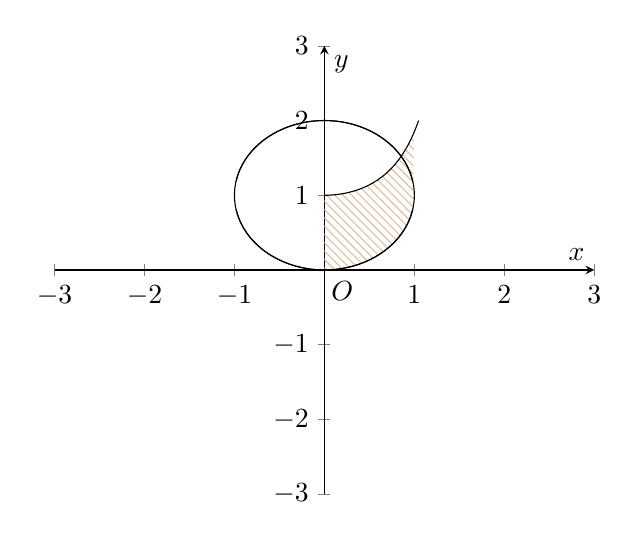
\begin{tikzpicture}
\begin{axis}
[
ymin=-3,ymax=3,
xmin=-3,xmax=3,
%clip=false,
xtick=\empty,
ytick=\empty,
extra x ticks={-3, -2, -1, 1, 2, 3},
extra y ticks={-3, -2, -1, 1, 2, 3},
axis lines = center,
xlabel=$x$,ylabel=$y$,
domain=-2.3:2.3,
samples=200,
]
\addplot [name path= C, black] {1 + sqrt(1 - x^2)};
\addplot [name path= D, black] {1 - sqrt(1 - x^2)};
\addplot [name path=L, black, domain=0:pi/3] {sec(deg(x))};
\addplot[pattern=north west lines, pattern color=brown!50]fill between[of=D and L, soft clip={domain=0:1}];
\node at (axis cs:0.2, -0.28) {$O$} ;
\draw (axis cs:0,1) circle [black, radius=1];
\end{axis}
\end{tikzpicture}
\end{document}
